\documentclass{scrartcl}
\usepackage{mm_ws15}

\newcommand{\sheetTitle}{Aufgaben, die nie gestellt wurden}
\begin{document}
\maketitle


\section{Das Methanmolekül}
Ein Methanmolekül (chemische Formel $\mathrm{CH}_4$) besitzt die Struktur eines regulären Tetraheders (siehe Bild).
Die Wasserstoffatome (weiß) befinden sich dabei in den Punkten $(0,0,0)$, $(k,k,0)$, $(k,0,k)$ und $(0,k,k)$; das Kohlenstoff im Zentrum im Punkt $(\frac{k}{2},\frac{k}{2},\frac{k}{2})$.
Hierbei bezeichnet $k$ eine Längenkonstante.
\begin{subex}
  \item Zeigen Sie, dass die angegebene Struktur tatsächlich einen regulären Tetraheder bilden, d.h.\ dass alle Verbingslinien zwischen den Wasserstoffatomen gleich lang sind.
  \item Berechnen Sie den Bindungswinkel zwischen zwei Wasserstoffatomen, d.h.\ den Winkel, der von zwei Wasserstoffatomen mit dem Kohlenstoffatom im Scheitelpunkt aufgespannt wird.
\end{subex}

\begin{center}
  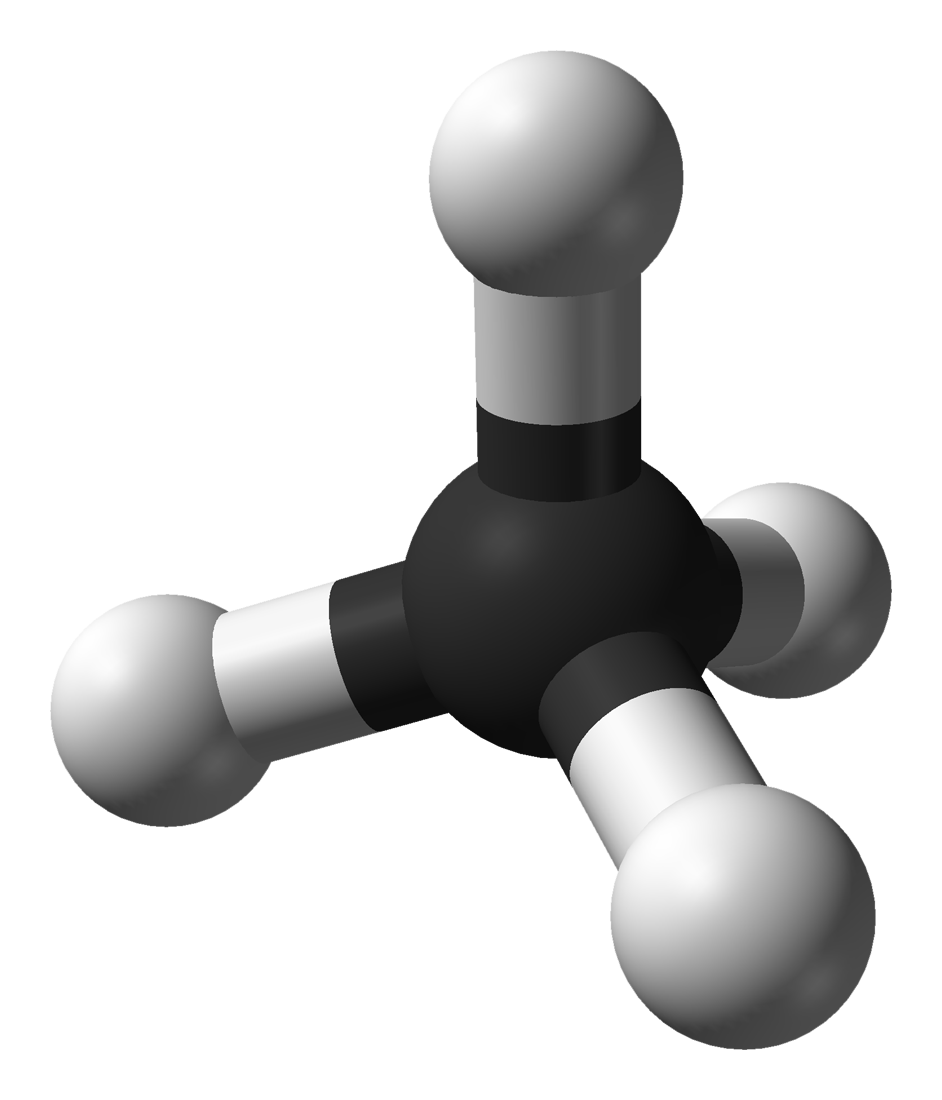
\includegraphics[width=3cm]{img/methan.png}
\end{center}


\end{document}
